\section{Секция 1}

\begin{itemize}
  \item \verb|Книга| имеющая название, том/часть, номер ISBN и количество экземпляров;
  \item \verb|Автор| определенный фамилией, именем, отчеством, авторским указателем;
  \item \verb|Зал| содержащий краткое название и полное название помещения;
  \item \verb|Стеллаж| с единственным атрибутом -- индекс стеллажа;
  \item \verb|Расположение| представляет собой связующей звено между \verb|Книгой|
  и \verb|Стеллажом|. Помимо технической информации содержит номера полок;
\end{itemize}

\begin{figure}[ht!]
  \begin{center}
    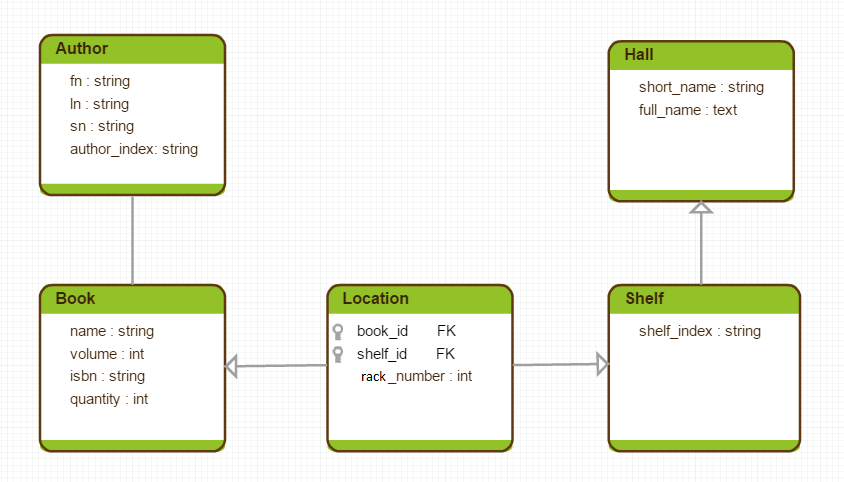
\includegraphics[scale=0.6]{images/erdiagramm.png}
  \end{center}
  \vspace*{-8mm}
  \caption{ER-диаграмма} \label{fig:erdiagramm}
\end{figure}

Вставка кода:
\begin{small}
  \begin{verbatim}
    rails g scaffold Book name:string volume:integer isbn:string quantity:integer
  \end{verbatim}
\end{small}

Вставка исходного кода:
\begin{small}
  \verbatiminput{programms/authors_migrate.rb}
\end{small}
